% Laboratorio de control, UDEA, Bioingeniería, 2025-2

\documentclass[journal]{IEEEtran} 

\IEEEoverridecommandlockouts

% *** Package
% *** Graphics package
\usepackage{graphicx}

% *** Math package 
\usepackage{amsmath}

% *** Float packages
\usepackage{float}

\usepackage{caption}
\captionsetup{
    justification=centering, % centra el caption
    font=footnotesize          % mantiene el tamaño pequeño del documento
}


\def\BibTeX{{\rm B\kern-.05em{\sc i\kern-.025em b}\kern-.08em
    T\kern-.1667em\lower.7ex\hbox{E}\kern-.125emX}}


    
\begin{document}

% paper title

\title{Sistemas Descritos en Función de Transferencia en S y Z}


\author{%%%% author names
    \IEEEauthorblockN{1\textsuperscript{st} Juan Esteban Campillo Zuluaga}% first author
    , \IEEEauthorblockN{2\textsuperscript{nd} Isabela Trujillo Betancourt},
    % delete this line if not needed
     \IEEEauthorblockN{3\textsuperscript{nd} Daniel Felipe Tamayo Cortes            }
    %%%% author affiliations
    \IEEEauthorblockA{\textit{Universidad de Antioquia Facultad de ingeniería, Bioingeniería, Teoría de control}}\\% first 
    
    %%%% corresponding author contact details
    \IEEEauthorblockA{juan.campillo@udea.edu.co, isabela.trujillob@udea.edu.co, danielf.tamayo@udea.edu.co}
}

\maketitle

\section{Introducción}

En el estudio de sistemas dinámicos, las funciones de transferencia constituyen una herramienta fundamental para describir matemáticamente la relación entre una entrada y la salida de un sistema. Estas permiten representar fenómenos fisiológicos, eléctricos o mecánicos de manera simplificada, facilitando el análisis en el dominio de Laplace y, posteriormente, en tiempo discreto mediante transformadas en z. En el contexto de la fisiología respiratoria, este enfoque resulta útil para comprender cómo variables como la presión, el volumen y el flujo se relacionan entre sí a través de modelos lineales aproximados.

En esta práctica se aplicaron estos conceptos mediante el uso de Python y la librería python-control, explorando tanto la simulación en tiempo continuo como la conversión de los modelos al dominio discreto. Para ello se trabajó con una entrada senoidal de presión (Pao) y se analizaron las respuestas de volumen y flujo del sistema respiratorio modelado. De manera general, el propósito de la práctica es fortalecer la comprensión de cómo los sistemas dinámicos pueden representarse y estudiarse a través de herramientas computacionales, integrando teoría y simulación para interpretar el comportamiento de un modelo fisiológico simplificado. 


\section{Información previa}

\subsection{Diagramas de bloques}
Los diagramas de bloques son representaciones gráficas que muestran cómo las señales fluyen a través de un sistema dinámico. Cada bloque representa una función matemática, normalmente una función de transferencia o relación entrada–salida, mientras que las flechas indican el sentido de las señales. Se utilizan porque permiten simplificar el análisis de sistemas complejos, visualizar la interconexión de sus componentes y aplicar de manera más clara las técnicas de control.

Lazo abierto: el sistema responde a una señal de entrada sin retroalimentación. Es decir, la salida no se mide ni se compara con la entrada. Ejemplo: encender un ventilador manualmente sin importar la temperatura de la habitación.

Lazo cerrado: la salida se mide y se retroalimenta hacia la entrada para reducir el error. Aquí existe un controlador que ajusta la señal de entrada según la diferencia entre lo deseado y lo obtenido. Ejemplo: un termostato que regula la temperatura de un cuarto activando o apagando el aire acondicionado

\subsection{Compliancia y resistencias en la mecánica respiratoria}



\begin{itemize}
    \item $R_c$: resistencia de la vía aérea central (por ejemplo, tráquea y bronquios principales).
    \item $R_p$: resistencia periférica de las vías aéreas más pequeñas.
    \item $C_L$: compliancia pulmonar (elasticidad del tejido pulmonar).
    \item $C_W$: compliancia de la pared torácica (elasticidad de la caja torácica).
    \item $C_S$: compliancia del sistema en conjunto, que integra pulmones y pared torácica.
\end{itemize}


La compliancia es la medida de la distensibilidad o capacidad de un sistema respiratorio para expandirse frente a un cambio de presión. Matemáticamente, se define como:

\begin{equation}
    C = \frac{\Delta V}{\Delta P}
\end{equation}

donde $\Delta V$ corresponde al cambio de volumen y $\Delta P$ al cambio de presión.

Su relevancia fisiológica radica en que determina la facilidad con que los pulmones y la caja torácica se expanden durante la respiración. Una compliancia reducida indica rigidez (como en la fibrosis pulmonar), mientras que una compliancia aumentada puede indicar pérdida de elasticidad (como en el enfisema).


\subsection{Simulación en Python}

\noindent
\textbf{Librerías utilizadas y su propósito:}

\begin{itemize}
    \item \textbf{python-control}: se utiliza para el modelado y análisis de sistemas dinámicos y de control. Permite crear funciones de transferencia, realizar simulaciones de la respuesta a entradas estándar (escalón, impulso, senoidal) y analizar estabilidad.
    
    \item \textbf{SciPy}: incluye herramientas avanzadas de integración numérica, resolución de ecuaciones diferenciales y optimización. Es fundamental para simular dinámicas de sistemas fisiológicos o de ingeniería.
    
    \item \textbf{NumPy}: proporciona estructuras de datos eficientes (como arreglos multidimensionales) y operaciones matemáticas de alto rendimiento. Es la base para el cálculo matricial y vectorial necesario en simulaciones.
    
    \item \textbf{Matplotlib}: se emplea para graficar resultados, como respuestas temporales, diagramas de Bode o espectros de señales. Permite visualizar claramente el comportamiento del sistema simulado.
\end{itemize}


\section{Resultados y discusión}

\subsection{Mécanica respiratoria}

\paragraph{Función de transferencia en el dominio continuo (S)}
La función obtenida para la mecánica respiratoria se evidencia en la ecuación \ref{eq:transferencia}

\begin{equation}
\scalebox{0.98}{$\frac{Q}{P_{ao}} = 
\frac{R_p C_s S^2 + \left(1 + \tfrac{C_s}{C_L} + \tfrac{C_s}{C_w}\right)S}
{R_c R_p C_s S^2
+ \left(R_c + R_p + R_c\tfrac{C_s}{C_L} + R_c\tfrac{C_s}{C_w}\right)S
+ \left(\tfrac{1}{C_L} + \tfrac{1}{C_w}\right)}$}
\label{eq:transferencia}
\end{equation}

El volumen se obtuvo al integrar la función de flujo, ya que el flujo es la derivada del volumen con respecto al tiempo. Esto equivale a multiplicar la función de flujo por 1/s en el dominio de Laplace.\bigskip

\paragraph{Simulación del modelo respiratorio en condiciones normales y patológicas}

En primer lugar, se simuló el sistema respiratorio en condiciones normales como se evidencia en la figura \ref{fig:simulacion_normal}, en esta se muestran los resultados de simulación obtenidos para el flujo de aire Q(t), y del volumen V(t) en respuesta a una presión de entrada Pao(t) (excitación sinusoidal) con una amplitud de 2,5 cm de H$_2$O a 15 respiraciones por minuto, lo cual corresponde a la frecuencia normal de respiración en reposo \cite{khoo2000physiological}. Como se puede observar en esta figura, la onda correspondiente al volumen se encuentra más en fase con Pao, mientras que el flujo de aire muestra un adelanto de fase con Pao. Adicionalmente, se puede evidenciar que el valor máximo alcanzado por la onda de flujo es de ~0,5, mientras que para el volumen es de ~0,4.

\begin{figure}[h!]
    \centering
    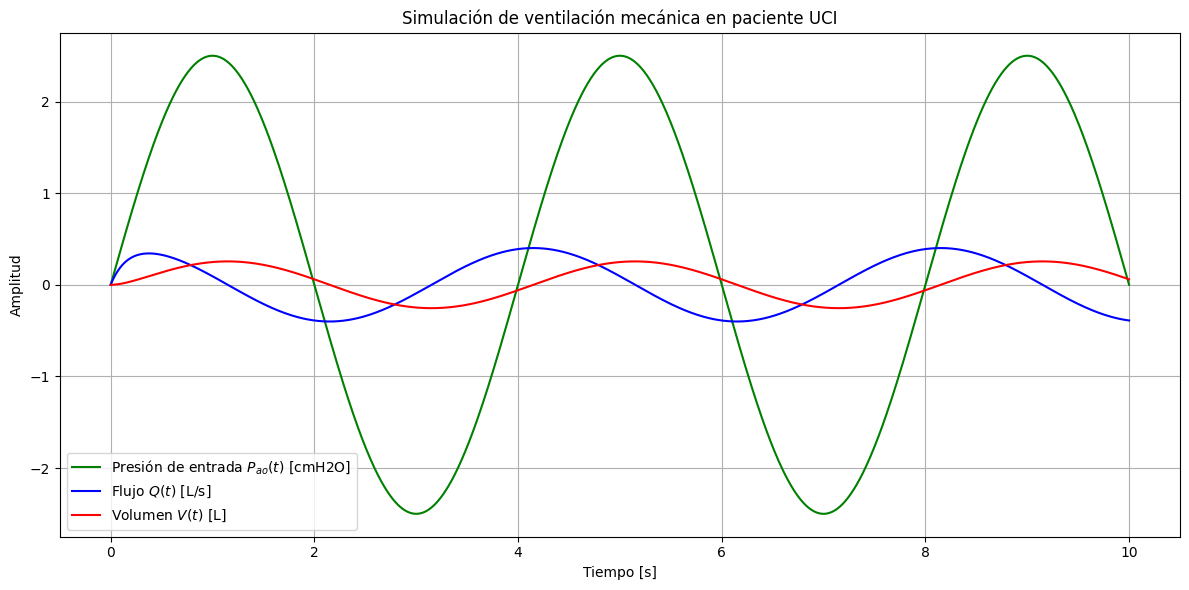
\includegraphics[width=1\linewidth]{Comportamiento-Practica1}
    \caption{Dinámica predicha del flujo de aire Q(t) y del volumen V(t) en respuesta a una excitación sinusoidal de Pao (amplitud = 2.5 cm H$_2$O) a 15 respiraciones por minuto}
    \label{fig:simulacion_normal}
\end{figure}

En segundo lugar, se procedió a simular el modelo respiratorio en tres diferentes casos de patologías, como se evidencia en la figura \ref{fig:comparacion}. 

\begin{figure}[H]
    \centering
    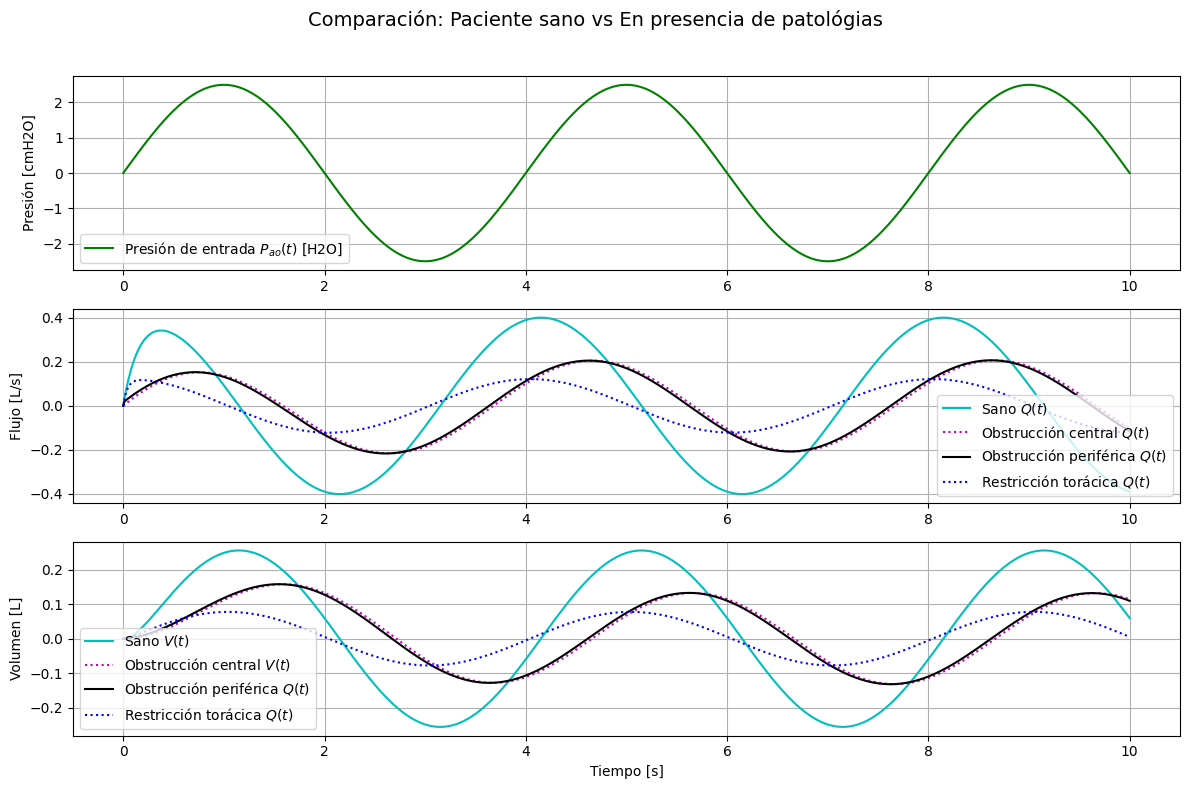
\includegraphics[width=1\linewidth]{Comparacion_Prac1.png}
    \caption{Comparación entre un paciente sano vs pacientes con patológias en su volumen y flujo de aire}
    \label{fig:comparacion}
\end{figure}

A continuación se expondrá cada patología simulada:\bigskip

•	\textbf{Obstrucción de la vía respiratoria central}:\\
La obstrucción de la vía respiratoria central (VRC) ocurre cuando hay un estrechamiento o bloqueo en estructuras como la tráquea, laringe o faringe. Esto impide el flujo normal de aire hacia los pulmones y puede ser potencialmente mortal si no se trata rápidamente \cite{mountsinai2023}. 

Por tal motivo, la resistencia de la vía respiratoria central se incrementa de manera significativa debido a la restricción del flujo aéreo, lo que ocasiona una disminución tanto del flujo inspiratorio como del volumen. En el modelo de circuito, este fenómeno se traduce en un aumento de la resistencia central (Rc). Para la simulación, se empleó un valor de 10, lo que corresponde a una enfermedad en grado 2 \cite{nguyen2010respiratory}.

Por ende, observamos en la figura \ref{fig:comparacion} como la curva tanto del volumen como del flujo disminuye su amplitud, lo cual indica que el pulmón no logra llenarse de manera adecuada. \bigskip

•	\textbf{Obstrucción de la vía respiratoria periférica}:\\
La vía respiratoria periférica incluye los bronquios pequeños, bronquiolos y alvéolos. La obstrucción en esta zona suele ser progresiva y difusa, y está asociada a enfermedades como:
\begin{itemize}
    \item EPOC (Enfermedad Pulmonar Obstructiva Crónica): incluye bronquitis crónica y enfisema \cite{nguyen2010respiratory}\cite{contreras2000epoc}
    \item Asma bronquial: obstrucción reversible por hiperreactividad bronquial \cite{nguyen2010respiratory}
\end{itemize}

En estas enfermedades se produce una inflamación crónica, lo cual provoca un engrosamiento de la pared bronquiolar. Esto hace que la resistencia aumente, ya que hay una oposición a la entrada del flujo aéreo, por tal motivo para simular esta patología se modificó la variable relacionada a la resistencia periférica (Rp), aumentandola a un valor de 10 para simular un paciente en grado 2 de la enfermedad \cite{nguyen2010respiratory}\cite{contreras2000epoc}. 

En la figura \ref{fig:comparacion}, se puede observar cómo la curva tanto del volumen como del flujo disminuyen en amplitud, teniendo un comportamiento similar al paciente que sufre de obstrucción en la vía respiratoria central, lo cual nos podría indicar que ambas enfermedades influyen de manera similar en el paciente; por consiguiente, se podría considerar que ambas resistencias inciden de forma semejante en la función de transferencia. \bigskip

•	\textbf{Restricción torácica}:\\
La restricción torácica forma parte del grupo de enfermedades pulmonares restrictivas extrapulmonares, donde el problema no está en el parénquima pulmonar sino en la estructura de la caja torácica o en los músculos respiratorios. Provocando una limitación mecánica para la expansión del tórax, lo que reduce la capacidad de los pulmones para llenarse de aire \cite{resmed2025restrictive}. 

Por tal motivo, hay una reducción de la distensibilidad torácica, lo que provoca un menor volumen inspirado. Esto se representó en la simulación variando el término correspondiente a la compliancia de la pared pectoral (Cw), disminuyendolo a 0.03 \cite{nguyen2010respiratory}.

En la figura \ref{fig:comparacion}, vemos como este valor afecta las curvas tanto del flujo como del volumen disminuyendo su pendiente de manera mucho más significativa que las otras dos enfermedades propuestas anteriormente, demostrando que la mecánica depende más de los efectos de la compliancia. Esta disminución en las amplitudes, nos indica que el volumen inspirado es menor y el flujo es reducido debido a la rigidez de la caja torácica, cumpliendo con lo que se espera de esta enfermedad. \bigskip


\paragraph{Conversión de la función de transferencia al dominio discreto (Z)}

Para la selección del tiempo de muestreo ($T_s$), se consideró la frecuencia de 15 respiraciones por minuto utilizada en la función de transferencia, lo cual equivale a una frecuencia de 0,25 Hz ($f$) o $\pi/2$ rad/s, como se muestra en la ecuación \ref{eq:freq}.

\begin{equation}
    f = \frac{15}{60} = 0.25 \,\text{Hz} = \frac{\pi}{2} \,\frac{\text{rad}}{\text{s}} \approx 1.57 \,\frac{\text{rad}}{\text{s}}
    \label{eq:freq}
\end{equation}

Este valor es relevante para la aplicación del teorema de Nyquist, el cual establece que una señal en tiempo continuo puede reconstruirse de manera exacta a partir de sus muestras siempre que la frecuencia de muestreo sea, como mínimo, el doble de la frecuencia máxima presente en dicha señal. De este modo, se evita la pérdida de información o distorsiones asociadas al aliasing \cite{academialab2025nyquist}.

De acuerdo con este principio, la frecuencia mínima de muestreo requerida para la correcta reconstrucción de la señal sería de 0,5 Hz. Sin embargo, en la práctica se recomienda emplear valores significativamente superiores, con el fin de capturar variaciones más sutiles y reducir posibles errores de reconstrucción. Por esta razón, en lugar de utilizar el doble de la frecuencia máxima, se decidió trabajar con un factor de 40 veces, obteniendo así una frecuencia de muestreo de 10 Hz, lo que corresponde a un período de muestreo de 0,1 s.

\subsection{Análisis del sistema continuo vs. sistemas discretos}

\paragraph{Función de transferencia en el dominio discreto}



\paragraph{Respuesta del sistema discreto ante diferentes entradas}


\begin{figure}[h!]
    \centering
    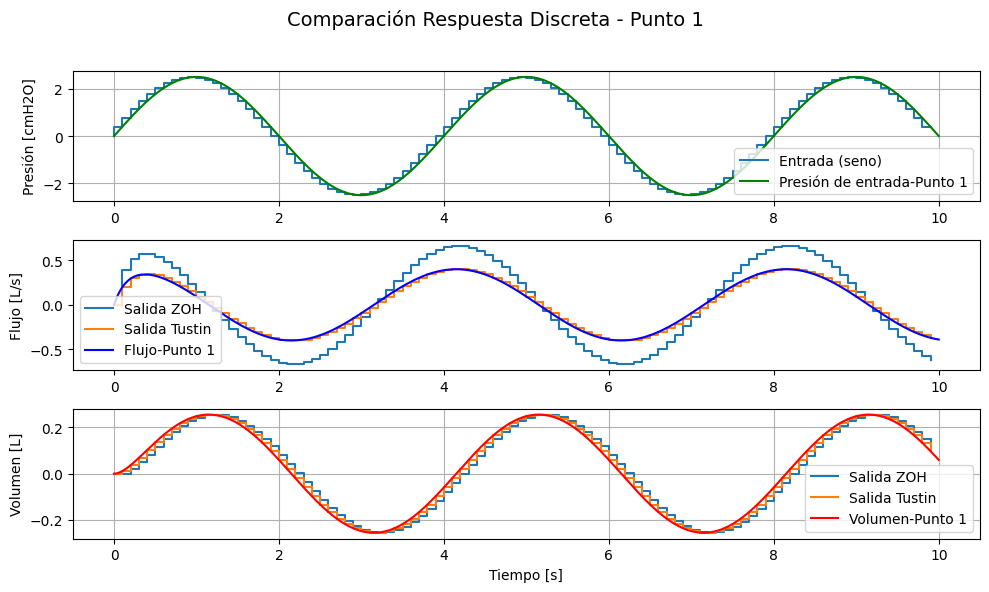
\includegraphics[width=1\linewidth]{Comparacion_P4.png}
    \caption{Comparacion entre las respuestas del sistema continuo vs sistema discreto en respuesta a una excitación sinusoidal.}
    \label{fig:simulacion_P4}
\end{figure}

\paragraph{Respuesta del sistema original continuo ante diferentes entradas}


\begin{figure}[h!]
    \centering
    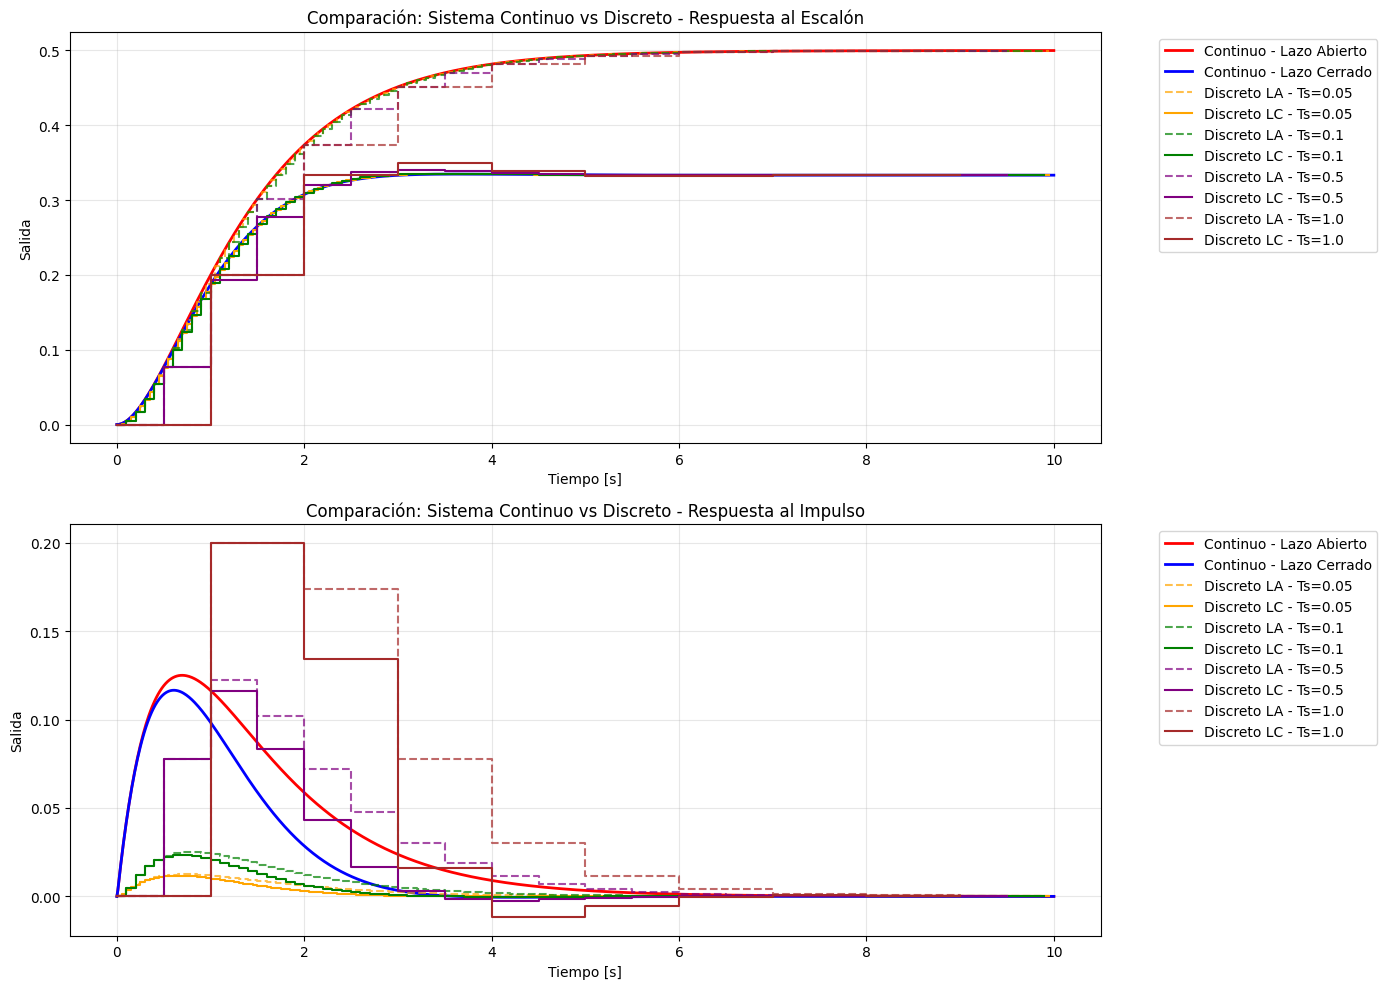
\includegraphics[width=1\linewidth]{Comparacion_P5.png}
    \caption{Comparacion entre las respuestas del sistema 2 en su forma continua vs sistema discreto variando el periodo de muestreo.}
    \label{fig:simulacion_P5}
\end{figure}


\section{Conclusiones}

% References

\bibliographystyle{ieeetr}   % estilo de bibliografía 
\bibliography{bibliografia-Pract1}  % nombre del archivo .bib SIN la extensión

\end{document}

